\chapter{Quantum computing for computational chemistry: NISQ devices} \label{Quantum computing for computational chemistry: NISQ devices}

\section{Noisy intermediate-scale quantum devices}
The acronym NISQ stands for 'noisy intermediate-scale quantum' devices and it is an expression coined by John Preskill in 2018 \cite{Preskill2018Aug}. It indicates quantum computers with a number of qubits ranging from 50 to a few hundreds, thus the term 'intermediate-scale'. 'Noisy' emphasizes that the control over these qubits is imperfect. Some of these devices are already available today and they are regarded as a step toward more powerful quantum technologies that will be developed in the future. \\
50 qubits is a significant milestone, because it is estimated to be beyond what can be simulated by brute force using the most powerful existing digital supercomputers, but, as we already mentioned, quantity is not the only important algorithmic parameter and quality must be considered and improved, i.e. longer coherence time, lower quantum noise and environment interactions and higher accuracy with which to perform quantum gates. \\
With these noisy devices researchers do not expect to be able to execute a circuit that contains many more than about 1000 gates, that is, 1000 fundamental two-qubit operations, because the noise will overwhelm the signal in a circuit much larger than that. This limitation on the circuit size imposes a ceiling on the computational power of NISQ technology. This condition can likely be improved only by using quantum error correction to scale up to larger circuits, meaning that when we speak of the NISQ era, we describe quantum computers with noisy gates, unprotected by quantum error correction. \\
\begin{figure}[ht]
  \centering
  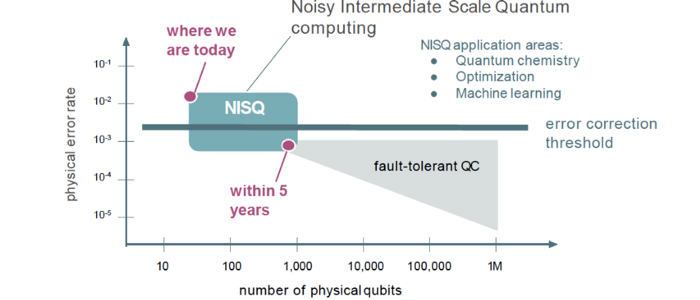
\includegraphics[width=\textwidth]{figures/NISQ.png}
  \caption{NISQ computing: error rate vs number of qubits.} \label{NISQ}
\end{figure} \\
A great component of the scientific debate on NISQ devices, and also on quantum computers, is if and when they will be able to solve important problems faster than classical computers and what type of problems. This condition is defined 'quantum speedup' and it considers using classical computers with the best available hardware and running the best algorithm which performs the same task. \\
Several research fields are considered better candidates for the first result to be shown using these devices, among these are: machine learning, optimization processes, linear algebra and simulation of quantum systems.

\section{Variational quantum eigensolver}
A highly researched algorithm for near-term quantum hardware is the variational quantum eigensolver (VQE), first proposed and experimentally realized by Alberto Peruzzo et al. \cite{Peruzzo2014Jul} and elaborated on by McClean et al. \cite{McClean2016Feb}. \\
The VQE aims to find the lowest eigenvalue of a given Hamiltonian, such as that of a chemical system, and is a hybrid quantum-classical algorithm. This means that it uses a quantum computer for state preparation, unitary evolution and measurement subroutine and it uses a classical computer to process the measurement results and update the quantum computer according to an specific rule. This exchanges the long coherence times needed for QPE for a overhead due to measurement repetitions and classical processing. \\
The VQE relies upon the Rayleigh-Ritz variational principle. This states that, for a parametrized trial wave function $|\Psi(\vec{\theta})\rangle$,
\begin{equation}
    \langle\Psi(\vec{\theta})|H|\Psi(\vec{\theta})\rangle \geq E_0,
\end{equation}
where $\vec{\theta}$ is a vector of independent parameters $\vec{\theta} = (\theta_1, ..., \theta_n)^T$. This implies that we can find the ground state wave function and energy by finding the values of the parameters which minimize the energy expectation value,
\begin{equation}
    E_{VQE} = min_{\vec{\theta}} \ \langle0| U^{\dagger}(\vec{\theta}) H U(\vec{\theta}) |0\rangle.
\end{equation}
As classical computers are unable to efficiently prepare, store and measure the wave function, we use the quantum computer for this subroutine. We then use the classical computer to update the parameters using an optimization algorithm. \\
\\
The scheme of the algorithm is:
\begin{enumerate}
    \item \textbf{Hamiltonian construction and representation} \\
    Here we define the system to study. We specify the geometry, find the specific operators and their weights between basis functions spanning the physical problem.
    
    \item \textbf{Encoding of operators} \\
    Qubit registers can only measure observables expressed in a Pauli basis. In second quantization we have fermionic operators, thus we need a transformation of fermionic operators to spin operators which mantain the antisymmetry as given by Pauli exclusion principle. This is also called fermionic-to-spin mapping or encoding. \\
    The key factors of an encoding are their Pauli weight, the number of qubits required and the number of Pauli strings produced.
    
    \item \textbf{Ansatz and state preparation} \\
    We prepare a trial wave function to measure the expectation value. For this we must decide on a structure for the parametrized quantum circuit, denoted as ansatz. \\
    A wide range of ansätze are possible, the key aspects are their expressibility and trainability. The former defines the ability of the ansatz to span a large class of states in the Hilbert space, the latter describes the practical ability of the ansatz to be optimized. These aspects are translated in terms of scaling and complexity of the circuit depth with system size.
    
    \item \textbf{Measurement strategy and grouping} \\
    We determine how measurements are distributed and organized to efficiently extract the required expectation values from the trial wave function. The objective of this component of the algorithm is to make the number of repetitions of the circuit as low as possible.
    
    \item \textbf{Parameter optimization} \\
    Here we update the parameters of the ansatz iteratively until convergence. This requires sampling the expectation value of the Hamiltonian several times for a given parameter set in the ansatz in order to define an update rule for the parameters.
    
    \item \textbf{Error mitigation} \\
    The VQE method is to be used without error correction schemes on NISQ devices. Error mitigation aims to reduce the impact of quantum noise through post-processing of the measurement data.
\end{enumerate}
The sequence of components is shown in Figure \ref{VQE scheme}. \\
In the following we analyze some important components of the VQE method: the encoding of operators, the ansatz and state preparation, the efficient grouping and measuring strategies and the error mitigation.
\begin{figure}[ht]
  \centering
  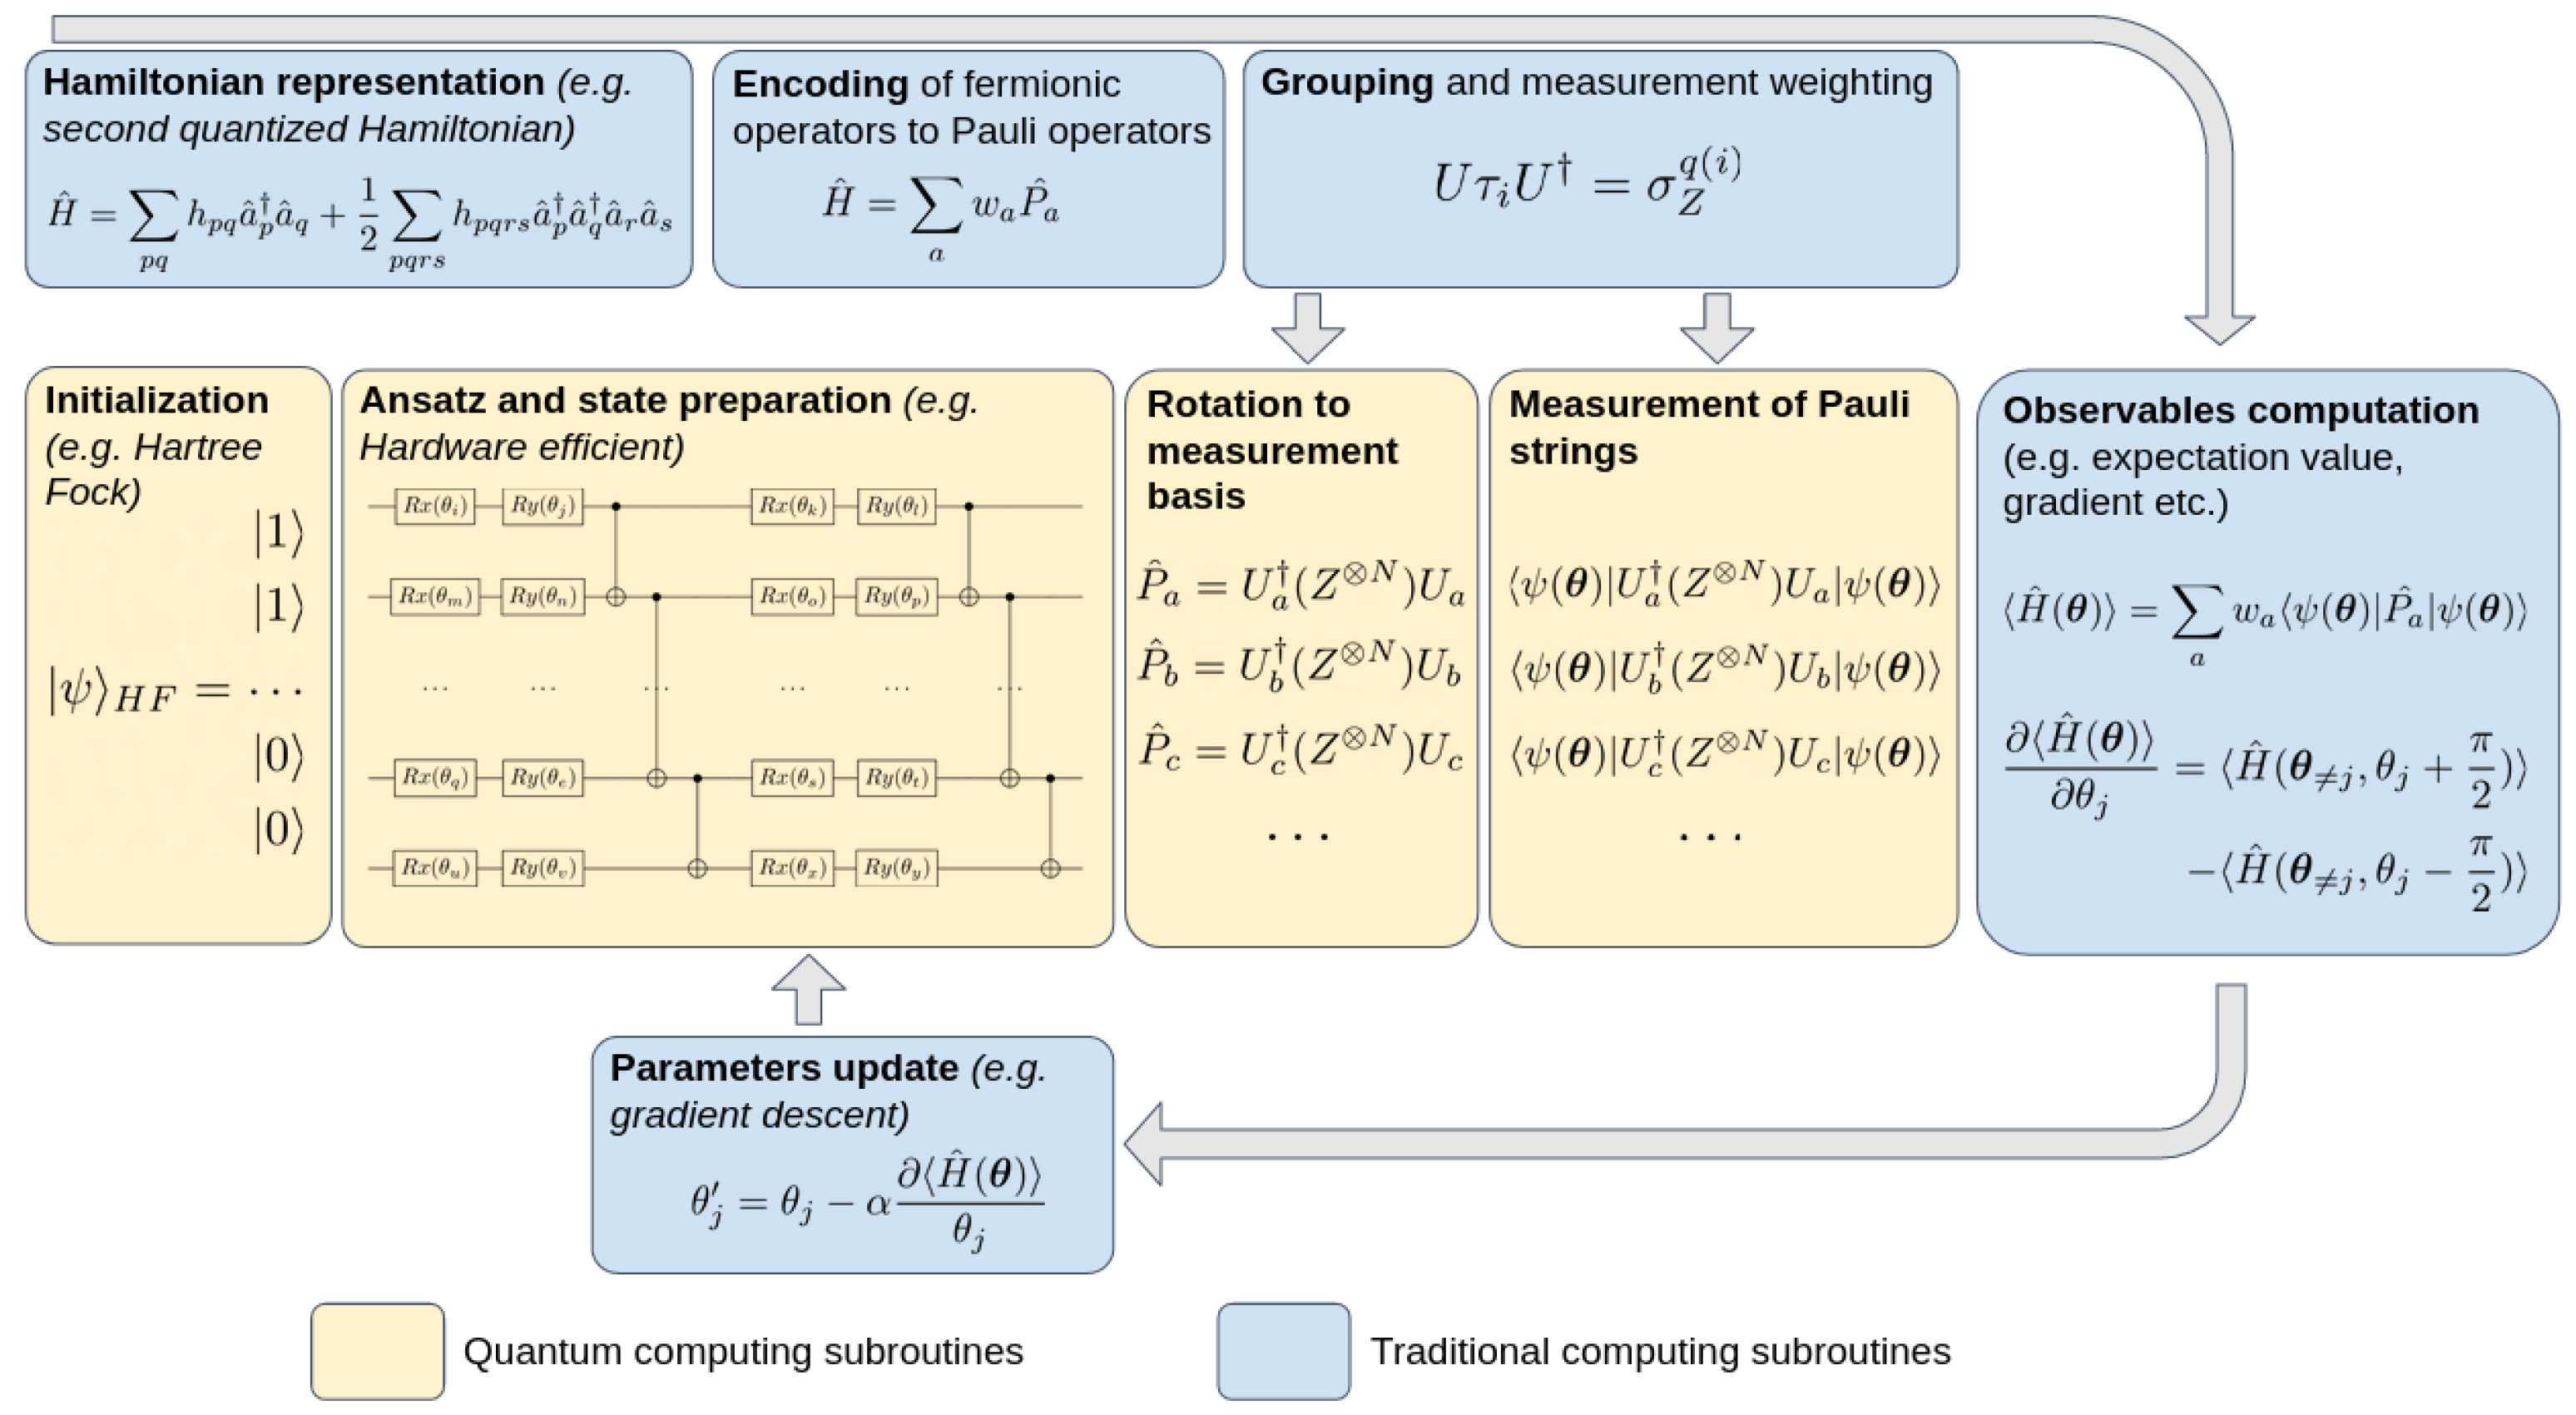
\includegraphics[width=\textwidth]{figures/VQE scheme.png}
  \caption{Flowchart for the VQE algorithm \cite{Tilly2021Nov}.} \label{VQE scheme}
\end{figure}

\subsection{Encoding of operators}
In the NISQ-era algorithms second quantization formalism has been favored over first quantization for quantum simulation. The fermionic creation and annihilation operators in second quantization formalism obey the anticommutative algebra. Qubits in comparison are spin-1/2 objects and, as such, the only operators that can be directly measured on quantum processors are spin operators, i.e. the Pauli operators $X$, $Y$, and $Z$, which obey a different algebra specified by their Lie bracket and do not naturally obey anticommutative rules. \\
All transformations between these two sets of operators can be formalized as
\begin{equation}
    \mathcal{T}: \mathcal{F}_n \rightarrow (\mathbb{C}^2)^{\otimes N},
\end{equation}
where a transformation $\mathcal{T}$ maps the space of operators acting on Fock states of $n$ orbitals, $\mathcal{F}_n$, to the Hilbert space $(\mathbb{C}^2)^{\otimes N}$ of operators acting on spin states of $N$ qubits. \\
The second quantized fermionic Hamiltonian is mapped to a linear combination of products of single-qubit Pauli operators
    \begin{equation}
        H = \sum_j w_j  P_j = \sum_j w_j \prod_i \sigma^j_i,
    \end{equation}
as already presented in Chapter \ref{Quantum computing for computational chemistry: FTQC devices}, where $w_j$ is the coefficient that correspond to the Pauli string $P_j$.
The mappings described here not only affect the operators measured when computing the expectation value of the Hamiltonian, but also the construction of an ansatz that is initially defined in fermionic terms. \\
There are three main features relevant to deciding on a specific encoding:
\begin{itemize}
    \item \textbf{The number of qubits required to represent the electronic wave function} \\
    In general, the number of qubits is directly proportional to the number of spin-orbitals or sites considered. However, several techniques have been developed to concentrate the information held in the wave function to as few qubits as possible.
    
    \item \textbf{The maximum number of qubits on which each produced Pauli string acts} \\
    This is the maximum number of non-identity operators in any Pauli string produced by the mapping and it is referred to as Pauli weight.
    It is important because low Pauli weigth results in lower depth ansätze and lower circuit construction costs, also it may provide resilience against the barren plateaus problem, i.e. a trainability problem that occurs in optimization algorithms when the gradient used to update the parameters $\vec{\theta}$ vanishes in every direction of the multidimensional space.
    
    \item \textbf{The number of different Pauli strings resulting from the mapping} \\
    In general, we see that this number of strings scales as $O(m^4)$ for molecular Hamiltonian and with the number of edges for lattice models.
\end{itemize}
Among the most used encodings are:
\begin{enumerate}
    \item \textbf{Jordan-Wigner encoding (JW)} \\
    This is a map that encodes the electronic wave function in an array of qubits by mapping the occupation number of spin-orbitals directly. \\
    The theoretical foundation of this mapping lies in the 1928 Jordan-Wigner transformation which uses spin-1/2 operators to explicitly describe fermionic ladder operators. \\
    We store the occupation number of a spin-orbital in the $\ket{0}$ or $\ket{1}$ state of a qubit. More formally,
    \begin{equation}
        \ket{n_0,n_1,...,n_i,...,n_{m-1}} \rightarrow \ket{q_0,q_1,...,q_i,...,q_{m-1}},
    \end{equation}
    \begin{equation}
        q_i = n_i \in \{ 0,1 \}.
    \end{equation}
    The fermionic creation and annihilation operators increase or decrease the occupation number of a spin-orbital by 1 and they also introduce a multiplicative phase factor. The qubit mappings of the operators preserve these features and are given by
    \begin{equation}
        a_i = \frac{X_i + iY_i}{2} \otimes Z_{i-1} \otimes ... \otimes Z_{0},
    \end{equation}
    \begin{equation}
        a^{\dagger}_i = \frac{X_i - iY_i}{2} \otimes Z_{i-1} \otimes ... \otimes Z_{0}.
    \end{equation}
    The operators $\frac{X_i \pm iY_i}{2}$ change the occupation number of the target spin-orbital, while the string of $Z$ operators recovers the exchange phase factor $(-1)^{\sum_k n_k}$. \\
    Working in the JW basis it is easy to see the advantage that quantum computers have over their classical counterparts for chemistry problems, since every Slater determinant required for the FCI wave function can be written as one of these computational basis states. As such, quantum computers can efficiently store the FCI wave function.
    However, while the occupation of a spin-orbital is stored locally, the parity is stored nonlocally. From the string of $Z$ operators we can see that a fermionic operator mapped to qubits generally has a weight of $O(m)$ Pauli operators, each acting on a different qubit.
    
    \item \textbf{Bravyi-Kitaev encoding} \\
    The Bravyi-Kitaev (BK) encoding is a midway point between the JW encoding and parity encoding methods because it compromises on the locality of the occupation number and the parity information. The orbitals store partial sums of occupation numbers and the occupation numbers included in each partial sum are defined by the BK matrix $\beta_{ij}$.
    \begin{equation}
        \ket{n_0,n_1,...,n_i,...,n_{m-1}} \rightarrow \ket{q_0,q_1,...,q_i,...,q_{m-1}},
    \end{equation}
    \begin{equation}
        q_i = \sum_j \beta_{ij} n_j \ (mod \ 2).
    \end{equation}
    The BK matrix is defined recursively via
    \begin{equation}
        \beta_1 = 1,
    \end{equation}
    \begin{equation}
        \beta_{2^{x+1}} = \left( \begin{array}{cc} \beta_{2^x} & \bf{0} \\
                                                   \bf{A} & \beta_{2^x} \end{array} \right),
    \end{equation}
    where $\bf{A}$ is a $2^x \times 2^x$ matrix of zeroes, with the bottom row filled with ones, and $\bf{0}$ is a $2^x \times 2^x$ matrix of zeroes. \\
    Applying the BK mapping to a fermionic operator results in a qubit operator with a Pauli weight of $O(log_2 m)$.
    
    \item \textbf{Optimal general encoding based on ternary trees} \\
    'Optimal' refers to the fact that for a Hamiltonian for which fermionic modes are fully connected it achieves the minimum average Pauli weight possible. It organizes qubits along with ternary trees and relies on the definition of the second quantized Hamiltonian in terms of Majorana fermions. \\
    Majorana fermions are theorized particles which acts as their own antiparticle. Formally this means that creation and annihilation operators for Majorana fermions are identical $\gamma^{\dagger}_i = \gamma_i$. These must anticommute if they are of different indices and commute otherwise. \\
    To build this encoding one must first map the qubits to the vertices of a ternary tree (a tree that splits into three edges after each vertex), as shown in Figure \ref{Ternary tree}. 
    \begin{figure}[ht]
    \centering
    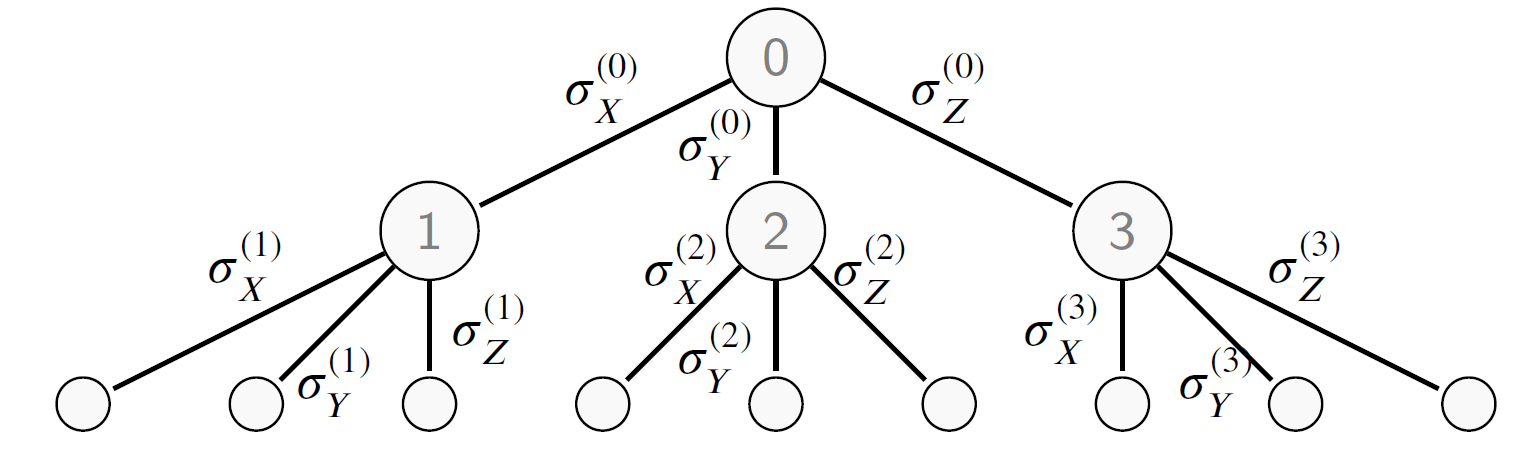
\includegraphics[width=0.8\textwidth]{figures/Ternary tree.png}
    \caption{Ternary tree structure in the case of a 4 fermionic modes system \cite{Tilly2021Nov}.} \label{Ternary tree}
    \end{figure} \\
    For any path $p$ in the tree one can define the following operators:
    \begin{equation}
        A_p = \bigotimes_{l=0}^{h-1} \sigma_{\alpha(l)}^{\nu(l)},
    \end{equation}
    where $h$ is the height of the tree, $\nu$ is the qubit index on path $p$ and $\alpha$ corresponds to $X$, $Y$ or $Z$, depending on whether the path follows the left, central or right edge respectively after qubit $\nu$. \\
    These operators clearly obey the same anticommutative relationships as Majorana operators. Given that there are $2n+1$ distinct path in the ternary tree and that we need $2n$ Majorana operators, we can map each $A_p$ to a single Majorana operator and these operators have a maximum Pauli weight equal to the height of the tree ($h$), hence $log_3(2n+1)$. \\
    To construct the Hamiltonian one needs to first transform the fermionic operators into Majorana operators and rewrite the Hamiltonian and then decide on an allocation of the Pauli operators defined above to the Majorana operators. Similar to the encodings defined previously defined, the number of qubits $n_q$ is equal to the number of fermionic modes $m$ and the scaling of the number of Pauli operators is the same as that of the two body-terms in the second quantized Hamiltonian $O(m^4)$.
\end{enumerate}

\subsection{Ansatz and state preparation}
The parametrized circuits, or ansätze, for the VQE lie between two extremes: hardware efficient and chemically inspired. There has been relatively little work comparing the effectiveness of different ansätze for anything but the smallest chemistry problems.
\begin{enumerate}
    \item \textbf{Hardware-efficient ansätze (HEA)} \\
    These ansätze are composed of repeated dense blocks of a limited selection of parametrized gates that are easy to implement with the available hardware. They seek to build a flexible trial state using as few gates as possible. As such, they are well suited to the quantum computers currently available, which have short coherence times and constrained gate topologies. However they are unlikely to be suitable for larger systems, as they take into account no details of the chemical system being simulated. \\
    A generic representation of HEA is
    \begin{equation}
        |\Psi(\vec{\theta)}\rangle = \left( \prod_{i=1}^d U_{rot}(\theta_i) \ U_{ent} \right) U_{rot}(\theta_{d+1}) \ket{\Psi_{in}},
    \end{equation}
    where $U_{rot}$ and $U_{ent}$ indicate a sequence of rotational and entangling gates. \\
    The main promise of hardware-efficient ansätze is that it can be flexibly tailored to the specific native gate set of the device used, while at the same time being highly expressive. \\
    The scaling of this method can be controlled by the number of layers $L$ of the circuit built, the depth scales as $n_g = O(L)$ and the number of parameters scales as $n_{rep} = O(m L)$.
    
    \item \textbf{Chemically inspired ansätze} \\
    Chemically inspired ansätze result from adapting classical computational chemistry algorithms to run efficiently on quantum computers. Most notably, the CC method discussed in Chapter \ref{Quantum computational chemistry} can be extended to produce the 'unitary coupled cluster' (UCC) ansatz \cite{Anand2022Mar}. \\
    The UCC method creates a parametrized trial state by considering excitations above the initial reference state and can be written as
    \begin{equation}
        U(\vec{\theta}) = e^{T-T^{\dagger}},
    \end{equation}
    where $T = \sum_i T_i$, and
    \begin{equation}
        T_1 = \sum_{i,\alpha} t_{i\alpha} a^\dagger_i a_\alpha,
    \end{equation}
    \begin{equation}
        T_2 = \sum_{i,j,\alpha,\beta} t_{i,j,\alpha,\beta} a^\dagger_i a^\dagger_j a_\alpha a_\beta, \ ...,
    \end{equation}
    $i,j$ indicate the occupied orbitals in the reference state and $\alpha,\beta$ indicate the orbitals that are initially unoccupied in the reference state. \\
    The UCC method is intractable on classical computers, but can be efficiently implemented on a quantum computer, as showed in the first description of the VQE algorithm by Peruzzo \cite{Peruzzo2014Jul}. \\
    A clear drawback of UCC-type ansätze is specifically that these are not hardware efficient. All UCC ansätze are designed in a manner that is agnostic to the connectivity of the device. The number of CNOT gates for each of the exponentiated Pauli strings required in the ansatz scales with its Pauli weight when full connectivity is allowed. Overall, this implies a very large prefactor for the depth and number of entangling gates of UCC anätze. \\
    \\
    For strongly-correlated systems, UCCSD may not be able to prepare a state which is suitably close to the ground state due to the limitation on the excitations considered. That is why an important extension of the UCC method can be used: the 'paired-UCC with generalized singles and doubles', k-UpCCGSD. This version is based on the paired-coupled cluster method, it only includes two-body terms that move pairs of electrons together between spatial orbitals. \\
    'Generalized' means that unlike conventional CC and UCC, which only include excitation operators that correspond to transitions from occupied to virtual orbitals, UCCG is agnostic to the electron configuration. \\
    Finally, k is a constant that indicates how many times the ansatz is repetead allowing more flexibility for the wave function description. \\
    The key advantage of this method is to allow a linear scaling ansatz, namely with $m$ the number of spin-orbitals, the ansatz depth scales $O(km)$, and a quadratic scaling in the number of parameters $O(km^2)$.
    
    \item \textbf{Adaptative structure ansätze} \\
    Adaptative structure ansätze aim to create a circuit structure tailored to the problem studied. As such they all work similarly: the ansatz is grown iteratively throughout the optimization process by adding new operators at each step based on their contribution to the overall energy estimate. \\
    The most simple is the ADAPT-VQE. Starting from an initial state, usually the Hartree-Fock wave function, and given a pool of operators $\{A_i\}$ the ADAPT-VQE ansatz evolves as follows, with the iteration number as superscripts:
    \begin{align}
        \ket{\Psi^{0}} & = \ket{\Psi_{HF}} \\
        \ket{\Psi^{1}} & = e^{\theta_1 A_1} \ket{\Psi_{HF}} \\
        \ket{\Psi^{2}} & = e^{\theta_2 A_2} e^{\theta_1 A_1} \ket{\Psi_{HF}} \\
        ... \\
        \ket{\Psi^{k}} & = \prod_i e^{\theta_i A_i} \ket{\Psi_{HF}}.
    \end{align}
    The operators in the pool are similar to those produced as part of the UCC ansatz, however, rather than specifying a number of possible excitation, one can include any one-, two body- or even higher body operator that is believed to be particularly relevant for the system considered. A good choice are the operators that result in the highest gradient of the energy functional with respect to the operator parameter.
\end{enumerate}
The k-UpCCGSD ansatz and its extensions have been numerically shown to achieve excellent accuracy while offering linear scaling, thereby arguably offering the best trade-offs of cost to accuracy among proposed ansätze. Adaptive ansätze could place themselves as a reliable alternative subject to further studies on their expected computational cost.

\subsection{Efficient grouping and measuring strategies}
One of the key challenges possibly holding back the VQE is the very large amount of samples that are required to accurately compute the relevant values of the algorithm. There are two main aspects to manage for efficiently sampling these expectation values: the number of terms in the Hamiltonian cost functions, computed using the mappings described before, and the number of shots required to sample an expectation value at a certain level of accuracy. \\
\\
First, let's consider the overall scaling of measurements, i.e. the number of shots. \\
As seen previously, generalized mappings for molecular Hamiltonians result in $P = O(m^4)$ distinct Pauli strings to estimate. \\
In any sampling experiment the standard error is equal to $\epsilon = \sigma / \sqrt{S}$, where $\sigma$ is the population standard deviation and $S$ is the experimental sample size, in our case the number of shots. This means that the number of times an experiment needs to be repeated to achieve a given expected error $\epsilon$ goes as $O(1/\epsilon^2)$. More specifically, when measurements are distributed optimally among the different Pauli strings, such that the variance is minimized with respect to a given precision $\epsilon$, the number of measurements required is upper-bounded by
\begin{equation}
S \leq \left( \frac{\sum_i^P w_i}{\epsilon} \right)^2,
\end{equation}
where $w_i$ are the weights of the Pauli strings in the Hamiltonian. \\
As a result, for a given level of accuracy for each Pauli string measured independently, the overall scaling of the number of shots required for an energy estimation is:
\begin{equation}
    S = O \left( \frac{m^4}{\epsilon^2} \right).
\end{equation}
In the context of quantum chemistry, successful computing methods are expected to produce results within a precision of $\epsilon = 1$ mHa to the target. When results obtained numerically are within this level of precision to experimental results the simulation is deemed to reach chemical accuracy. \\
One should be cautious however not to assume too much of a relationship between this number and the number of shots required to perform VQE. That is because the key bottleneck of VQE optimization is not the estimation of the wave function itself but the estimation of gradients and in particular the difference between these gradients. While polynomial in scaling, it has been pointed out on several occasions that the number of shots required to accurately compute a VQE optimization process rapidly becomes unmanageable.

\begin{enumerate}
    \item \textbf{Qubit-wise commutativity (QWC)} \\
    Two Pauli strings are said to be QWC if each Pauli operator in the first string commute with the Pauli operator of the second one that has the same index. Generally speaking, that would be any group where any given Pauli operator in any Pauli string has an index such that all the operators of the same index across all the other Pauli strings in the group are either the same Pauli operator or the identity (for example, $XI$, $IZ$, and $XZ$ are altogether QWC). \\
    This basis for grouping terms has been widely used and studied. It allows performing joint measurements more efficiently. In particular, Gokhale et al. \cite{Gokhale2019Jul} found that this method reduces the prefactor for the number of Pauli terms to be measured by about three, without however changing its asymptotic scaling. \\
    Another key advantage is that the basis rotation used to conduct the joint measurements only requires a circuit of depth 1. To achieve this, we need to find the unitary which rotates all the Pauli strings in a given QWC group into a basis in which they are all diagonalized. This is a straightforward process as any individual Pauli operator can be rotated in the Z basis with one single-qubit operation as follows:
    \begin{equation}
        Z = R_y\left( -\frac{\pi}{2} \right) X R_y\left( -\frac{\pi}{2} \right)^{\dagger},
    \end{equation}
    \begin{equation}
        Z = R_x\left( \frac{\pi}{2} \right) Y R_x\left( \frac{\pi}{2} \right)^{\dagger}.
    \end{equation}
    This method of grouping and joint measurement is therefore relatively cheap to implement and allows for significant savings in the number of shots required to complete a VQE, although without changing the overall scaling.
    
    \item \textbf{Basis rotation grouping} \\
    Basis rotation grouping is based on a tensor decomposition of the two-body operators. It reduces the overall number of joint terms to measure in the Hamiltonian, down to a linear number with system size. This same decomposition has also been used to reduce the total gate depth of the full UCCSD ansatz as well as the Trotter steps. It also provides a large improvement in the noise resilience of mappings with high Pauli weight such as Jordan-Wigner. \\
    The price to pay for this is that the measurement has to take place in a different basis for each term, necessitating an additional $O(m)$ gate depth before measurement to implement this orbital rotation for each grouped term of this decomposed Hamiltonian.
\end{enumerate}
The definition of the ’best possible grouping method’ is not straightforward. While it is clear that aiming for the lowest number of groups possible is advantageous, it is not the only metric to take into consideration. In particular, it was shown that grouping terms suffers from covariances arising from the joint measurement. This covariance effects increase the
sampling noise and as such the total number of measurements required to achieve a given level of precision, which should be taken into consideration as figure of merit for a grouping strategy. \\
Another cost to consider is the additional quantum noise resulting from the circuit used to rotate the measurement basis, since further resources may be required to mitigate these additional errors.

\subsection{Error mitigation}
As we mentioned before, when the noise of a quantum computer is below a certain threshold and a sufficient number of qubits are available, quantum error correction schemes can be applied to suppress the noise to arbitrarily small levels, however this brings different types of overheads, including large amounts of extra ancilla qubits, fast decoding and communication between quantum and conventional devices. \\
As an alternative, a series of techniques for mitigating the effects of noise for quantum algorithms running on NISQ hardware have been developed. These techniques have been shown to achieve a reduction in noise levels on expectation value estimates, without requiring the large resources involved in error correction. Such methods are be critical for early implementations of the VQE algorithm in order to achieve the required precision for quantum chemistry computation. \\
These techniques are effective only when used with low-depth circuits such that the total error rate in the circuit is low. However, the additional resources required are much more modest than those for full error correction. In general, these techniques require only multiplicative overhead in the number of measurements needed if the error rate is sufficiently low. \\
As we are dealing with errors, it becomes necessary to consider mixed states rather than just pure states, thus we have to use the density matrix formalism of quantum mechanics. \\
A general output state where each gate is affected by a noise channel $\mathcal{N}_i$ is
\begin{equation}
    \rho = \prod_i \mathcal{N}_i \circ \mathcal{U}_i (\ket{0}\bra{0}),
\end{equation}
and the output without the noise is
\begin{equation}
    \rho_0 = \prod_i \mathcal{U}_i (\ket{0}\bra{0}),
\end{equation}
where, for a density matrix $\rho$ it is true that $\mathcal{U}_i(\rho) = U \rho U^{\dagger}$ and the result of the measurement of a Hermitian observable $O$ on this state is
\begin{equation}
    \bar{O} = Tr(\rho O).
\end{equation}
The error mitigation methods can approximate the noiseless measurement result $\bar{O}_0$ from the noisy measurement result $\bar{O}$ when the error rate is sufficiently low. It is important to note that error mitigation schemes are not a scalable solution to the problem of noise in quantum hardware. In order to scale up computations to arbitrarily large-size, fault-tolerant, error-corrected quantum computers are required.
\begin{enumerate}
    \item \textbf{Extrapolation} \\
    The extrapolation method works by intentionally increasing the dominant error rate $\epsilon_0$ by a factor $\lambda$, and inferring the error-free result by extrapolation. \\
    The technique is based on Richardson extrapolation, which to first order corresponds to linear extrapolation using two points. We could also take a linear or higher order fit with several data points. For the former case, the estimated value of the observable is given by
    \begin{equation}
        \bar{O}_0^{est} = \frac{\lambda \bar{O}(\epsilon_0) - \bar{O}(\lambda \epsilon_0)}{\lambda - 1}.
    \end{equation}
    While this method can improve the accuracy of calculations, it requires additional measurements in order to keep the variance of the measured observable the same as in the non-extrapolated case. \\
    An alternative is the exponential extrapolation which was introduced as a more appropriate extrapolation technique for large quantum circuits.
    
    \item \textbf{Probabilistic error cancellation} \\
    This method works by effectively realizing the inverse of an error channel, $\mathcal{N}^{-1}$, such that $\mathcal{N}^{-1} [ \mathcal{N} (\rho_0) ] = \rho_0$. \\
    Because realizing the inverse channel is in general an unphysical process, we use the scheme depicted in Figure \ref{Probabilistic error cancellation} to effectively realize the inverse channel by focusing only on measurement results.
    \begin{figure}[ht]
    \centering
    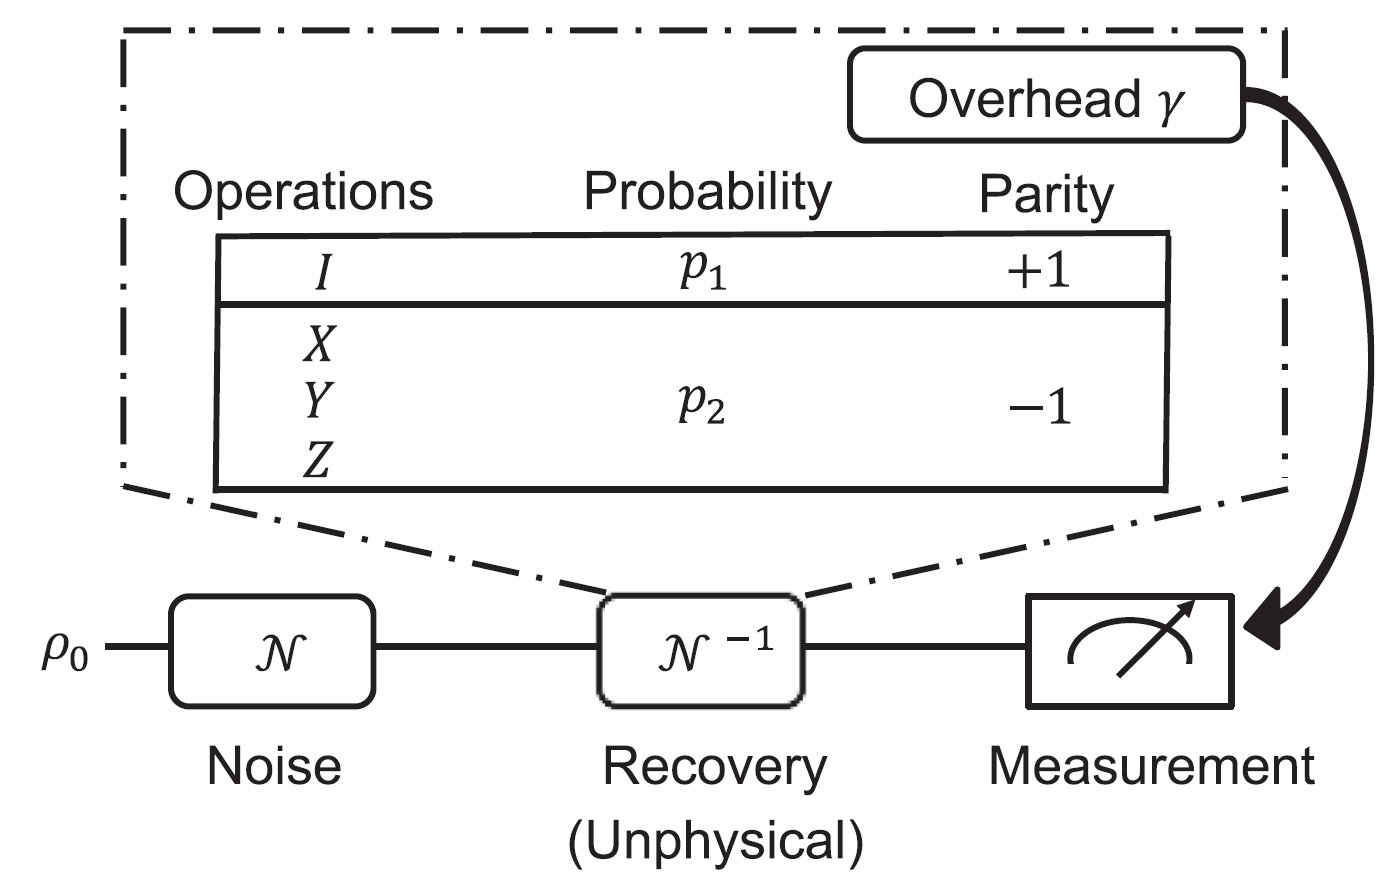
\includegraphics[width=0.6\textwidth]{figures/Probabilistic error cancellation.png}
    \caption{Probabilistic error cancellation method for a depolarizing error \cite{Tilly2021Nov}.} \label{Probabilistic error cancellation}
    \end{figure} \\
    For example in a depolarizing error channel the unphysical inverse channel is
    \begin{equation}
        \rho_0 = \mathcal{D}^{-1}(\rho) = \gamma [p_1\rho - p_2(X\rho X + Y\rho Y + Z\rho Z)].
    \end{equation}
    However, we can consider and correct its effect on the expectation value $\bar{O}_0$,
    \begin{align}
        \bar{O}_0 & = Tr[O\mathcal{D}^{-1}(\rho)] \\
        & = \gamma [p_1 \langle O \rangle_{\rho} - p_2(\langle O \rangle_{X\rho X} + \langle O \rangle_{Y\rho Y} + \langle O \rangle_{Z\rho Z})] \\
        & = \gamma [p_1 \langle O \rangle_{\rho} - p_2(\langle O \rangle_{\rho} + \langle O \rangle_{\rho} + \langle O \rangle_{\rho})],
    \end{align}
    where $\langle O \rangle_{\rho} = Tr[O\rho]$. We can therefore measure $O$, $XOX$, $YOY$, and $ZOZ$ and linearly combine the measurement results to effectively realize the inverse channel, thus obtaining the noiseless measurement result $\bar{O}_0$. \\
    In practice, it is not possible to exactly measure all of the possible terms resulting from errors if there are many gates in the circuit. Instead, we can consider only the most important terms, which result from a small number of errors occurring. If the error rate is low, then the other terms can be considered negligibly small. \\
    After each single-qubit gate we can apply $X$, $Y$ or $Z$ operators with probability $p_2$ or the identity gate with $p_1$. We repeat that circuit variant many times to extract the expectation value and multiply the expectation value by $(-1)^{G_p}$ , where $G_p$ is the number of additional $X$, $Y$ or $Z$ gates that were applied in that circuit iteration. We then sum up the values for several circuit variants and multiply by $\gamma$ to obtain the error mitigated result. This method can also be extended to multiple-qubits gates. \\
    Probabilistic error cancellation requires full knowledge of the noise model associated with each gate. This can be obtained from either process tomography or a combination of process and gate set tomography. The latter approach reduces the effect of errors due to state preparation and measurement.
    
    \item \textbf{Quantum subspace expansion} \\
    The quantum subspace expansion (QSE) can mitigate errors in the VQE, in addition to calculating the excited energy eigenstates. This method is most effective at correcting systematic errors, but it can also suppress some stochastic errors. Suppose that we use the VQE to find an approximate ground state $|\tilde{E}_0\rangle$. Noise may cause this state to deviate from the true ground state $|E_0\rangle$. For example, if $|\tilde{E}_0\rangle = X_1|E_0\rangle$ we can simply apply an $X_1$ gate to recover the correct ground state. \\
    However, as we do not know which errors have occurred, we can instead consider an expansion in the subspace $\{ |P_i \tilde{E}_0 \}$, where $P_i$ are matrices belonging to the Pauli group. Then one can measure the matrix representation of the Hamiltonian in the subspace
    \begin{equation}
        H^{QSE}_{ij} = \langle\tilde{E}_0|P_iHP_j|\tilde{E}_0\rangle.
    \end{equation}
    As the subspace states are not orthogonal to each other we should also measure the overlap matrix
    \begin{equation}
        S^{QSE}_{ij} = \langle\tilde{E}_0|P_iP_j|\tilde{E}_0\rangle.
    \end{equation}
    Then, by solving the generalized eigenvalue problem
    \begin{equation}
        H^{QSE} C = S^{SQE} C E,
    \end{equation}
    with a matrix of eigenvectors $C$ and diagonal matrix of eigenvalues $E$, we can get the error mitigated spectrum of the Hamiltonian. A small number of Pauli group operators are typically considered in order to minimize the required number of measurements \cite{McArdle2020Mar}.
\end{enumerate}

\section{Computational requirements}
Analogously to Chapter \ref{Quantum computing for computational chemistry: FTQC devices} we give an estimate of the computational requirements for the VQE with one example. \\
Again the algorithmic parameters that we consider are:
\begin{itemize}
    \item \textbf{circuit width ($n_q$)}
    
    \item \textbf{circuit depth ($n_g$)}
    
    \item \textbf{repetitions ($n_{rep}$)}
    
    \item \textbf{total scaling ($n_t = n_g \cdot n_{rep}$)}
\end{itemize}
The number of qubits needed to represent the relevant quantum states is generally equal to the number of spin-orbital,
\begin{equation}
    n_q = O(m).
\end{equation}
This is the case for both the Jordan-Wigner and Bravyi-Kitaev transformations. It is, however, typically possible to reduce this number slightly by conserving symmetries of the chemical system. \\
The number of times the circuit must be repeated will be the product of two factors: the number of circuit applications or shots, $S$, required to obtain a single estimate of the Hamiltonian expectation and the number of Hamiltonian expectations, $n_h$, required in order to optimize the parameters so that 
\begin{equation}
    n_{rep} = S \cdot n_h.
\end{equation}
To find these we first consider the ansatz. \\
The choice of the circuit plays a key role in determining the performance of a VQE calculation. The ideal ansatz would:
\begin{itemize}
    \item \textbf{Enable preparation of a state close to the true ground state;}
    
    \item \textbf{Require as few parameters as possible,} so as to minimise the time required to perform the classical optimization;
    
    \item \textbf{Use as few quantum computational resources as possible.}
\end{itemize}
In general the ansatz circuit depth will depend on the accuracy, $\epsilon$, as a deeper circuit will typically allow a state closer to the true ground state to be prepared. However, it is difficult to quantify the relationship between $n_g$ and $\epsilon$. Here, we first consider a fixed ansatz: the UCCSD ansatz. \\
The key property of the ansatz that affects the VQE calculation time is the number of parameters, $n_p$. For the UCCSD ansatz, this is
\begin{equation}
    n_p = O(n_e^2 (m - n_e)^2) \sim O(m^4),
\end{equation}
which is the scaling of the number of $t_{i,j,\alpha,\beta}$ parameters, where $n_e$ indicates the number of electrons considered. \\
The number of Hamiltonian expectations required in a particular VQE calculation is difficult to know in advance as it will depend on the shape of the ansatz parameter space. Here we assume that this number, $n_h$, is simply given by
\begin{equation}
    n_h = n_p.
\end{equation}
This, for example, could arise if the optimizer need only to look in each parameter direction once, perhaps to verify that a minimum has already been found. Needing any fewer evaluations would imply that it was known before the calculations occurred that some parameters were not needed in the ansatz. Typical calculations will require more evaluations than this. \\
The number of applications of the ansatz circuit needed depends on the form of the Hamiltonian and the particular quantum state. Measurements of Pauli operators can easily be obtained, thus, assuming that each one of these is obtained separately, the number of times the ansatz circuit must be performed is given by
\begin{equation}
    S = \left( \frac{1}{\epsilon} \sum_i |w_i| \sqrt{Var[P_i]} \right)^2, \label{number of measurements}
\end{equation}
where $\epsilon$ is the desired error in the expectation estimate, $w_i$ is the coefficient of the Pauli string $P_i$ and
\begin{equation}
    Var[P_i] = 1 - \langle \psi(\vec{\theta}) |P_i| \psi(\vec{\theta}) \rangle.
\end{equation}
The maximum value of each variance is 1 and so
\begin{equation}
    S \leq \left( \frac{E_{max}}{\epsilon} \right)^2,
\end{equation}
as we saw before, where again $E_{max} = \sum_i |w_i|$. \\
In the following we take the equality in this expression. \\
We note that it is possible to reduce this through several different measuring strategies, such as those described before. It is possible to improve upon the assumption that we measure each Pauli individually by, for example, measuring commuting Pauli operators simultaneously or factorising the two-electron integral tensor. Such methods reduce the overall number of measurements required whilst retaining the scaling in $\frac{1}{\epsilon^2}$. This scaling can also be improved using QPE-inspired methods at the cost of an increased circuit depth. However, such increased depths are unlikely to be possible in the NISQ era, before error correction is available. \\
For the circuit depth we assume that it is possible to perform $n_q$ parameters per layer
of gates and so
\begin{equation}
    n_g = O(m^3)
\end{equation}
for the UCCSD ansatz. \\
In conclusion, the algorithmic parameters scale as \cite{Blunt2022Jun}
\begin{equation}
    n_q^{VQE} = O(m), \ n_g^{VQE} = O(m^3), \ n_{rep}^{VQE} = O \left( \frac{m^4 E_{max}^2}{\epsilon^2} \right) \label{Scaling VQE}
\end{equation}
Likewise QPE we consider $E_{max}$ scaling between $O(m)$ and $O(m^3)$ \cite{Lee2020Nov}. \\
Thus the the total scaling for the VQE algorithm is
\begin{equation}
    n_t^{VQE} = n_g^{VQE} \cdot n_{rep}^{VQE} = O \left( \frac{E_{max} m^7}{\epsilon^2} \right). \label{Scaling VQE 1}
\end{equation}
Moreover, J. Tilly et al. \cite{Tilly2021Nov} presented the sequence of components for the VQE algorithm which offer the most promising scaling without compromising excessively on accuracy for molecular systems and lattice models. \\
The key distinctive factor separating molecular systems and lattice models is that the former makes no assumption on the range and type of interaction between the fermionic modes, beyond it being a two-body interaction, while the latter usually has a simplified and parameterized form which often only connects fermionic modes following a nearest-neighbor lattice structure and/or features a lower effective rank of interactions. \\
Here the list of components:
\begin{enumerate}
    \item \textbf{Hamiltonian construction} \\
    Molecular system: Second quantization - $O(m^4)$ Hamiltonian terms and $O(m)$ number of qubits; \\
    Lattice models: Second quantization - $O(m^4)$ Hamiltonian terms and $O(m)$ number of qubits;
    
    \item \textbf{Fermion to spin encoding} \\
    Molecular system: Ternary tree encoding - $O(n_q^4)$ operators and $O(log_3(2n_q))$ Pauli weight; \\
    Lattice models: Generalized superfast encoding - $O(md/2)$ qubits, with $d$ the fermionic-interaction graph maximum degree, $O(ND)$ operators, with $D$ the lattice dimension, and $O(log_2(d))$ Pauli weight;
    
    \item \textbf{Ansatz} \\
    Molecular system: k-UpCCGSD - $O(kn_q)$ circuit depth and $O(kn_q^2)$ parameters; \\
    Lattice models: Hamiltonian variational ansatz (HVA) - $O(k\tilde{C})$ circuit depth and parameters, with $\tilde{C}$ the number of commutative groups in the Hamiltonian;
    
    \item \textbf{Grouping and measurement strategy} \\
    Molecular system: Decomposed interactions - $O(n_q)$ operators to measure and $O(n_q/2)$ additional basis rotation circuit depth; \\
    Lattice models: Qubit-wise commutation - $O(1)$ operators to measure and additional basis rotation circuit depth;
    
    \item \textbf{Optimizer} \\
    Molecular system: Rotosolve - requires sampling three values for each parameter at each step; \\
    Lattice models: Rotosolve - requires sampling three values for each parameter at each step;
    
    \item \textbf{Error mitigation strategy} \\
    Molecular system: Symmetry verification and extrapolation based methods - exponential with respect to the circuit depth; \\
    Lattice models: Symmetry verification and extrapolation based methods - exponential with respect to the circuit depth;
\end{enumerate}
Now we describe the total scaling of such a sequence of components. \\
The computation of the expectation value of a single operator at a precision $\epsilon$, which would cover the same range as chemical accuracy, requires $O(1/\epsilon^2)$ repetitions of the ansatz. If the k-UpCCGSD ansatz is chosen this scales as $O(km)$ \cite{Lee2019Jan}, while choosing to use the decomposed interactions requires $O(m)$ different operators to be measured and therefore a gate depth of $O(m)$ for rotation to the joint measurement basis, resulting in a total scaling for a single estimation of the entire Hamiltonian of $O(km^2/\epsilon^2)$. \\
There are $O(km^2)$ parameters in the k-UpCCGSD ansatz \cite{Lee2019Jan}, hence this represents the cost scaling of updating each parameter using the Rotosolve optimizer. As this optimizer is not parallelizable one may prefer to use a different method if sufficient sets of qubits are available. Overall, this gives a total scaling for one iteration of the VQE of
\begin{equation}
    n_t^{VQE} = O\left( \frac{k^2m^4}{\epsilon^2} \right) \label{Scaling VQE 2}
\end{equation}
without parallelization, and
\begin{equation}
    n_t^{VQE} = O(km)
\end{equation}
with full parallelization for the circuit depth. \\
This example shows how different ansätze can lead to very different scalings for and how research on better components of an algorithm can improve scaling even by several orders of magnitude. \\
\\
A perfect parallelization would require $O(km^3/\epsilon^2)$ sets of $O(m)$ qubits. Note that while qubits within one set need to be entangled for the course of a single measurement, there is no requirement for entanglement between qubits of different sets of parallel quantum computers nodes. The sets of qubits can therefore be either all within one quantum computer, or else also distributed across different separated quantum computers. \\
So far we have only considered the scaling of one iteration. It is still an open research question how the number of iterations required to achieve convergence scales with system size for the VQE. This depends on numerous factors, including the ansatz, the optimizer used and the system studied. One important point to note is that convergence tends to be rapid at the beginning of the optimization process, with large gradients that require only a low number of shots to be computed accurately enough to progress. It becomes more challenging close to the optimum, where gradients are smaller, requiring a larger number of shots to continue the optimization. As such the last few iterations of the VQE are likely orders of magnitude more expensive than the rest of the optimization, if the algorithm is implemented efficiently.

\subsection{Example}
Several studies estimated the resource requirements for NISQ approaches. The majority stand on the statement that the VQE method leads to a number of measurements and repetitions needed to simulate industrially-relevant systems that are prohibitively large. However, we discuss more on this in Chapter \ref{Computational advantage}. \\
\\
One example is the study by J. Gonthier et al. \cite{Gonthier2020Dec} who, in 2020, estimated the number of qubits, number of measurements and total runtime required for calculating combustion energies for small organic molecules to within chemical accuracy with a single VQE energy evaluation. These estimates consider the so-called 'frozen natural orbitals' (FNO) as well as measurement reduction techniques such as Hamiltonian term grouping, application of fermionic marginal constraints and low-rank factorization of the Hamiltonian. \\
They considered a benchmark set of organic molecules, shown in Figure \ref{Organic molecules}, and studied their combustion reactions, whose general formula is:
\begin{equation}
    C_xH_yO_z + \left( x + \frac{y}{4} - \frac{z}{2} \right) O_2 \leftrightharpoons xCO_2 + \frac{y}{2}H_2O.
\end{equation}
\begin{figure}[ht]
  \centering
  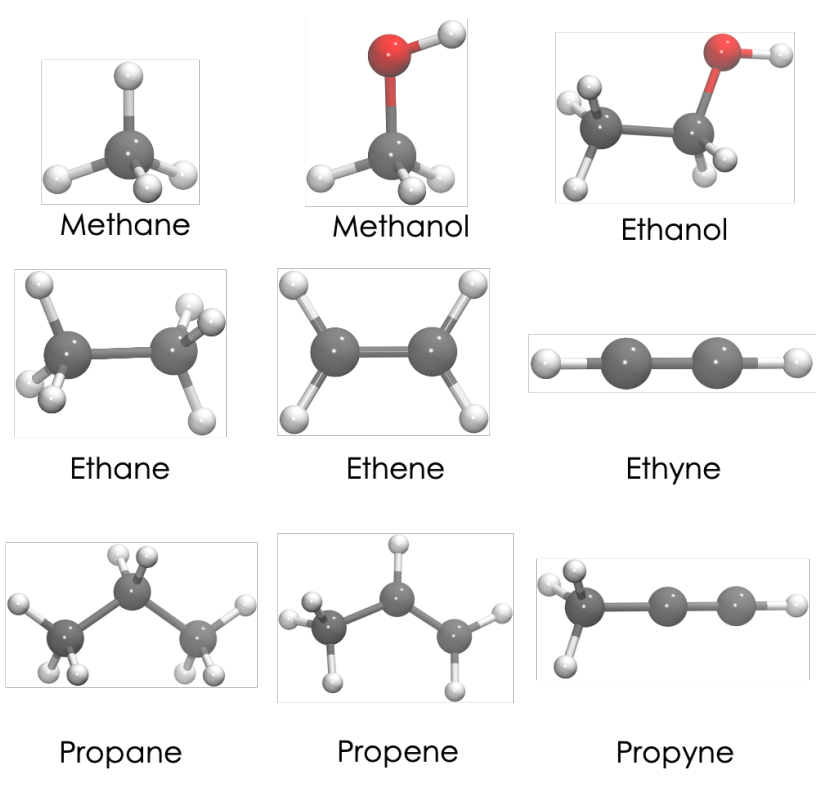
\includegraphics[width=0.55\textwidth]{figures/Organic molecules.png}
  \caption{Benchmark set of rganic molecules \cite{Gonthier2020Dec}.} \label{Organic molecules}
\end{figure} \\
First, they benchmarked classical chemistry methods reaching the conclusion that the performance of common methods that can routinely be applied to larger systems is insufficient to reach chemical accuracy, although it improves with larger basis set, and to get even better results the very resource-demanding coupled cluster method is needed. \\
\\
The quantum computation part was executed on the Zapata Computing's Orquestra workflow management platform. \\
For the scaling in depth only the number of measurements is considered. \\
The formula to estimate this number, $M$, is
\begin{equation}
    M = \frac{K}{\epsilon^2},
\end{equation}
where $K$ is the Hamiltonian variance and is defined as
\begin{equation}
    K = \left( \sum_C \sqrt{\sum_{\alpha, \beta \in C} w_{\alpha} w_{\beta} Covar(P_{\alpha}, P_{\beta}) } \right)^2,
\end{equation}
which is analogous to eq. (\ref{number of measurements}), with $P_i$ the Pauli operators and $w_i$ their coefficients. \\
They evaluated $K$ for QWC grouping and basis rotation approach with two different basis for the Hamiltonian (canonical orbitals or FNOs) and two different estimates for the variances (upper bounds or CISD), giving a total of 4 different settings for each grouping method. \\
They ran computations for all molecules in the set and also included H$_2$O and CO$_2$, that are necessary for computing combustion energies. \\
For each molecule they computed different active spaces with an integer number of
qubits per active electron up to a total of 80 qubits. Then they fit the results to a power law for each grouping method:
\begin{equation}
    K = a(n_q)^b.
\end{equation}
The results are shown in Figure \ref{K values}.
\begin{figure}[ht]
  \centering
  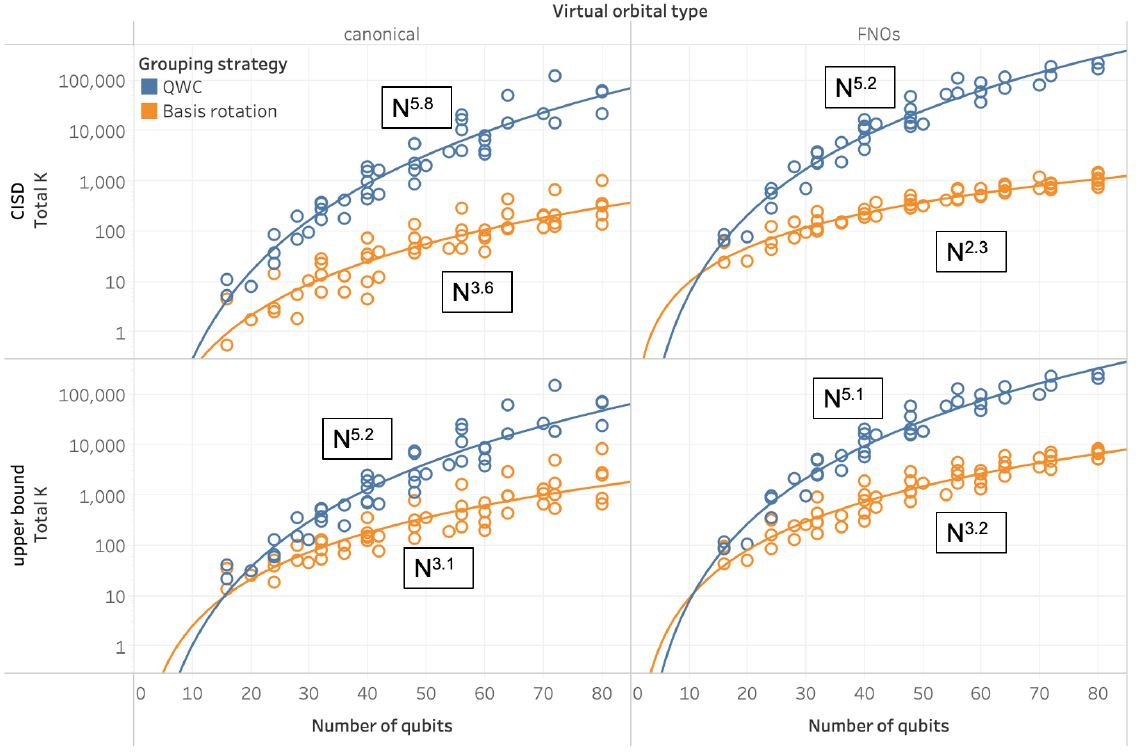
\includegraphics[width=\textwidth]{figures/Values of K for QWC and basis rotation grouping.png}
  \caption{Values of $K$ for QWC and basis rotation grouping, with $K = a(n_q)^b$ \cite{Gonthier2020Dec}.} \label{K values}
\end{figure} \\
The number of terms in the quantum chemistry Hamiltonian scales as $O(n_q^4)$, as we have seen before. However, the QWC grouping method with optimal measurement allocation approximately scales between $O(n_q^5)$ and $O(n_q^6)$. Thus, the observed scaling for QWC grouping only constitutes a modest improvement over the estimated upper bound of $O(n_q^6)$ for scaling without grouping.
Basis rotation grouping offers significantly better scaling. This varies between $O(n_q^{2.3})$ and $O(n_q^{3.6})$, a very significant improvement compared to QWC grouping results. In addition, the effect of this improved scaling is already beneficial at low number of qubits, so that QWC grouping never appears advantageous in the computed data. \\
For the number of qubits they used $n_q \approx 13 n_{el}$, where $n_{el}$ is the number of electrons. This comes from using FNO as a basis set with which to model the atomic orbitals. \\
\\
Finally, for the runtime they assumed to use a shallow hardware-efficient ansatz, a linear connectivity of the qubit array, in which case a single layer is defined as the circuit of depth 2 that entangles every neighboring pair of qubits, and assumed that the number of layers needed to reach the ground state energy scales linearly with the number of qubits. \\
Considering the runtime dominated by execution times of two-qubit gates, assumed to be 100 ns (a value on the faster side of current superconducting gate times), the final formula used to obtain runtimes $t$ in seconds is
\begin{equation}
    t = 10^{-7} M (5n_q - 3).
\end{equation}
The results for the different molecules are reported in Figure \ref{VQE scaling 1}, with $\epsilon = 0.5$ mHa.
\begin{figure}[ht]
  \centering
  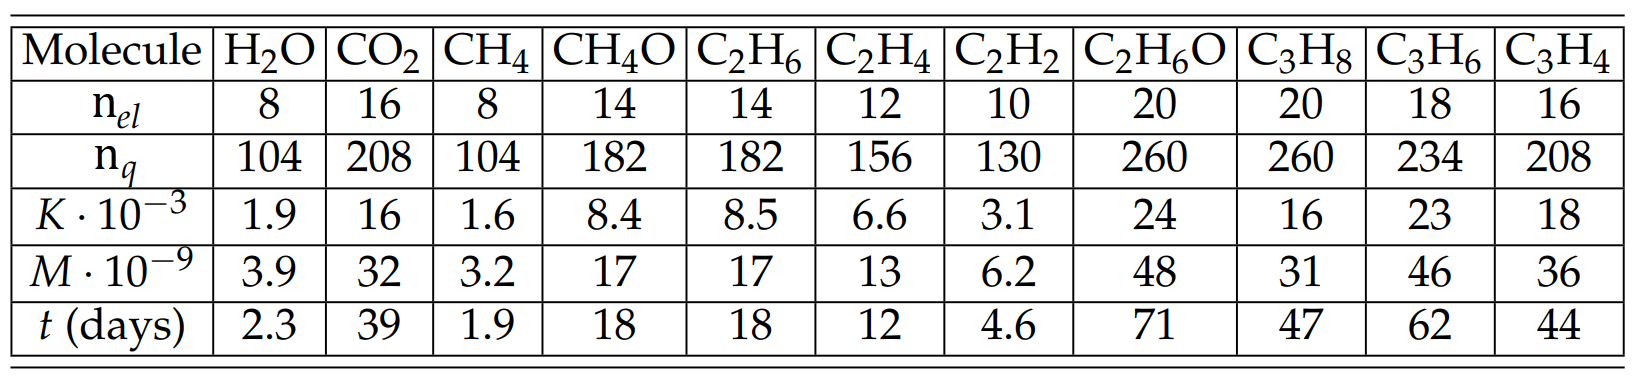
\includegraphics[width=0.9\textwidth]{figures/VQE scaling 1.png}
  \caption{Estimated runtimes for a single energy evaluation \cite{Gonthier2020Dec}.} \label{VQE scaling 1}
\end{figure} \\
Moreover, they highlighted that this is the time necessary for a single energy evaluation and that running the full VQE algorithm involves optimizing the circuit parameters, which requires at least a few dozen to hundreds of iterations even with excellent optimizers. Hence, the total VQE runtime would be about a month for the smallest molecules in this test set.